% Chapter 6 (Utility Evaluation)

\chapter{Utility Evaluation: No Synthesis versus Dynamic Tool Synthesis}
\label{ChapterEval}
\lhead{Chapter 6. \emph{Utility Evaluation}}
\sloppy

\section{Experimental Setup}
The utility pillar of the evaluation protocol (\fref{fig:evaluation_pillars}) compares
agents limited to generic execution capabilities with agents that can register and
reuse dynamically synthesized tools. The evaluation
is implemented as a self-contained TypeScript harness in the \texttt{experiments/}
directory of the repository, built on the Vercel AI SDK and its \texttt{dynamicTool()}
primitive for runtime-registered tools \cite{aisdk}. All conversations run on
\texttt{deepseek-v4-pro} \cite{deepseek}, a reasoning-enabled model.

Five experiments cover three domains. SQL and parser synthesis are each tested with
repetitive and mixed workloads; a third, software-engineering domain tests repeated
repository configuration audits:

\noindent\textbf{SQL domain.} An airline customer-service agent answers passenger
cancellation requests over a deterministic, seeded SQLite database of seven tables
(\texttt{passengers}, \texttt{bookings}, \texttt{booking\_segments}, \texttt{flights},
\texttt{tickets}, \texttt{payments}, \texttt{refund\_requests}; 150 passengers, 220
bookings). Every cancellation question requires joining all seven tables --- roughly
one page of SQL. The agent is told nothing about the schema in advance.

\noindent\textbf{Parser-synthesis domain.} An operations analyst extracts cancellation
events from six daily operations-log exports written in a hostile legacy text format:
\texttt{key=value} fields in arbitrary order, quoted values containing commas, amounts
in mixed USD/EUR with a per-file exchange rate in the header, and comment/heartbeat
noise lines. No SQL is involved. Scripts execute in a \texttt{node:vm} sandbox with
explicit inputs, an explicit capability allow-list (a scoped \texttt{readFile(name)}),
a one-second timeout, and bounded output --- mirroring IronClaw's execution envelope.

\noindent\textbf{Repository-compliance domain.} A software supply-chain agent audits
six repository snapshots against seven deterministic policies spanning dependency
versions, production secrets, container users and health checks, mutable CI action
references, Node.js versions, and production debug settings. Each repository contains
\texttt{package.json}, a \texttt{Dockerfile}, a GitHub Actions workflow, and a production
environment file. This domain uses neither SQL nor logs.

The \textbf{repetitive} workloads (E1, E3, E5) issue six requests that all
require the same query, parser, or audit logic with different inputs; the \textbf{mixed} workload
(E2, E4) repeats it in only three of six requests, the rest being one-off questions.
Following Chapter~\ref{Chapter4}, metrics per request are: billed input/output tokens
(summed over all model steps, i.e.\ what the provider actually charges), reasoning
tokens, cached input tokens, model steps (turns), tool calls, characters of code
(SQL or JavaScript) the model had to author, wall-clock time, and answer correctness
(verified against ground truth).

\section{Scenario Design}
Two scenarios share each domain's generic base capabilities and differ only in whether
the repeated artifact can be registered for reuse (\tref{tab:scenarios}).

\begin{table}[htbp]
    \centering
    \caption{Utility evaluation scenarios (instantiated per domain).}
    \label{tab:scenarios}
    \small
    \begin{tabular}{@{}clp{9.5cm}@{}}
        \toprule
        \textbf{ID} & \textbf{Label} & \textbf{Beyond the base tools} \\
        \midrule
        A & No synthesis & Generic query or sandboxed-script capabilities only; the agent authors the required task logic inline for every request. \\
        B & Dynamic synthesis & The same generic capabilities plus a meta-tool and explicit policy to register the repeated logic once and reuse it. \\
        \bottomrule
    \end{tabular}
\end{table}

This is the comparison tested by H1: no synthesized tool versus a dynamically created
tool, with identical data, requests, model, and generic capabilities.

\section{Results: SQL Domain}
\tref{tab:e1_totals} reports E1 totals; \tref{tab:e1_steady} the steady state
(requests 2--6), excluding the one-time schema discovery all agents perform on
request 1.

\begin{table}[htbp]
    \centering
    \caption{E1 (SQL, repetitive) totals over six requests (deltas relative to A).}
    \label{tab:e1_totals}
    \small
    \begin{tabular}{@{}lrr@{}}
        \toprule
        \textbf{Metric} & \textbf{A: no synthesis} & \textbf{B: dynamic synthesis} \\
        \midrule
        Input tokens        & 190{,}031 & 88{,}566 ($-$53.4\%) \\
        Output tokens       & 6{,}783   & 5{,}526 ($-$18.5\%) \\
        \quad of which reasoning & 1{,}654 & 1{,}977 \\
        Code authored (chars)& 3{,}142  & 1{,}800 ($-$42.7\%) \\
        Model steps         & 28        & 15 ($-$46.4\%) \\
        Tool calls          & 45        & 15 ($-$66.7\%) \\
        Wall time           & 103.6\,s  & 81.3\,s ($-$21.5\%) \\
        \bottomrule
    \end{tabular}
\end{table}

\begin{table}[htbp]
    \centering
    \caption{E1 (SQL, repetitive) steady state: average per request, requests 2--6.}
    \label{tab:e1_steady}
    \small
    \begin{tabular}{@{}lrr@{}}
        \toprule
        \textbf{Metric (avg/request)} & \textbf{A: no synthesis} & \textbf{B: dynamic synthesis} \\
        \midrule
        Input tokens  & 35{,}183 & 14{,}840 ($-$57.8\%) \\
        Output tokens & 1{,}000  & 691 ($-$30.8\%) \\
        Code authored & 510\,chars & 0 ($-$100\%) \\
        Wall time     & 15.3\,s  & 10.3\,s ($-$33.0\%) \\
        \bottomrule
    \end{tabular}
\end{table}

Dynamic synthesis halves billed input tokens relative to no synthesis
($-$53.4\%), and in the steady state answers each passenger with a single two-step
tool call authoring \emph{zero} code, while A re-authors the query (or a chain of
smaller ones) on every request. After the one-time creation step, B authors no SQL on
repeats and reduces steady-state model input by 57.8\%.

In E2 (mixed workload), only requests 1, 3, and 5 repeat the lookup. The creation
overhead is not recovered: B lands at +19.0\% input tokens relative to A
(87{,}442 vs.\ 73{,}452) with output tokens essentially unchanged ($-$5.0\%).
Synthesis, in other words, does not pay off in the SQL domain at this repetition
level.

\section{Results: Parser-Synthesis Domain}
E3/E4 replace the SQL artifact with a JavaScript parser and the database with bulk
log text. One design detail proved decisive: in an initial configuration where
created tools received the full file text as a parameter, every call pushed bulk data
through the conversation and synthesis was net-negative (+12\% input). Allowing the
sandbox to load data itself through a session capability (\texttt{readFile(name)} ---
the same allow-listed capability the agent has) made tool inputs tiny and flipped the
result. \tref{tab:e3_totals} reports the final configuration.

\begin{table}[htbp]
    \centering
    \caption{E3 (parser, repetitive) totals over six requests (deltas relative to A).}
    \label{tab:e3_totals}
    \small
    \begin{tabular}{@{}lrr@{}}
        \toprule
        \textbf{Metric} & \textbf{A: no synthesis} & \textbf{B: dynamic synthesis} \\
        \midrule
        Input tokens        & 193{,}817 & 74{,}865 ($-$61.4\%) \\
        Output tokens       & 8{,}757   & 3{,}606 ($-$58.8\%) \\
        \quad of which reasoning & 4{,}244 & 1{,}011 ($-$76.2\%) \\
        Code authored (chars)& 6{,}109  & 1{,}196 ($-$80.4\%) \\
        Model steps         & 18        & 13 ($-$27.8\%) \\
        Tool calls          & 12        & 7 ($-$41.7\%) \\
        Wall time           & 91.7\,s   & 47.2\,s ($-$48.5\%) \\
        \bottomrule
    \end{tabular}
\end{table}

The pattern replicates --- and strengthens. B reduces billed input tokens by 61.4\%
and, notably, reasoning tokens by 76.2\%: offloading parsing to deterministic code
removes most of the model's per-request reasoning.

E4 (mixed workload) replicates the SQL break-even finding more strongly: B lands at
+64.7\% input tokens (106{,}131 vs.\ 64{,}452). With only two reuses of the created
parser, the creation transcript inflates the history carried by every later request.

\section{Results: Repository-Compliance Domain}
E5 tests the same mechanism on a software-engineering task rather than data access or
log parsing. All six requests apply the same seven compliance rules to different
repository snapshots. Both scenarios identified every seeded violation and produced
the correct severity counts.

\begin{table}[htbp]
    \centering
    \caption{E5 (repository compliance, repetitive) totals over six requests.}
    \label{tab:e5_totals}
    \small
    \begin{tabular}{@{}lrr@{}}
        \toprule
        \textbf{Metric} & \textbf{A: no synthesis} & \textbf{B: dynamic synthesis} \\
        \midrule
        Input tokens         & 140{,}472 & 65{,}146 ($-$53.6\%) \\
        Output tokens        & 12{,}429  & 4{,}826 ($-$61.2\%) \\
        \quad of which reasoning & 1{,}911 & 538 ($-$71.8\%) \\
        Code authored (chars)& 29{,}176 & 9{,}112 ($-$68.8\%) \\
        Model steps          & 19 & 13 ($-$31.6\%) \\
        Wall time            & 134.0\,s & 61.4\,s ($-$54.2\%) \\
        \bottomrule
    \end{tabular}
\end{table}

In the steady state (requests 2--6), dynamic synthesis reduced average input tokens
from 27{,}276 to 12{,}270 ($-$55.0\%), output tokens from 2{,}049 to 583
($-$71.6\%), authored code from 4{,}818 to 901 characters ($-$81.3\%; the remaining
code is the one-time registration on request 2), and wall time from 21.6 to 7.7 seconds
($-$64.4\%). Requests 3--6 required no further authored audit code.

\begin{figure}[htbp]
    \centering
    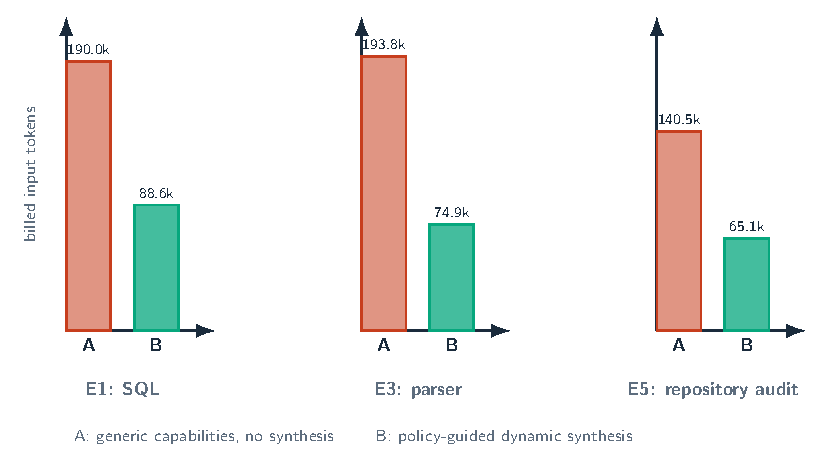
\includegraphics[width=0.98\linewidth]{Figures/fig_utility_tokens.pdf}
    \caption{Billed input tokens for no synthesis (A) and dynamic synthesis (B). Repetitive workloads (E1, E3, E5) save 53--61\%; mixed workloads (E2, E4) are net-negative.}
    \label{fig:utility_tokens}
\end{figure}

\section{Findings}
Across three domains and five experiments, the utility evaluation supports six findings:
\begin{enumerate}[label=\textbf{F\arabic*.}, leftmargin=1.6cm]
    \item \textbf{On repetitive workloads, dynamic tool synthesis is decisively
    cheaper than authoring artifacts inline} --- $-$53.4\% (SQL), $-$61.4\%
    (parser), and $-$53.6\% (repository compliance) billed input tokens, with
    identical correctness.
    \item \textbf{The benefit extends to software-engineering work.} E5 reduces
    model steps by 31.6\%, authored code by 68.8\%, and wall time by 54.2\%.
    \item \textbf{Payoff scales with reuse; below the threshold it is a net cost.}
    At three-of-six repetitions, synthesis landed at +19.0\% (SQL) and +64.7\%
    (parser) input tokens.
    \item \textbf{The enabling condition is tool-side data access.} Tools must take
    small lookup keys and load data behind the tool boundary; passing bulk data
    through the conversation as tool arguments erased the benefit in the parser
    domain (+12\% vs.\ $-$61\% after the capability fix).
    \item \textbf{Synthesis offloads reasoning, not just tokens.} Reasoning tokens
    dropped 76.2\% in E3 and 71.8\% in E5 because deterministic tools substitute
    for repeated model reasoning.
    \item \textbf{Runtime tool registration is per-step.} A tool created
    mid-generation only becomes callable at the next model step; the harness steps
    the tool loop explicitly, and platforms with meta-tools must do the same.
\end{enumerate}

All final answers in A and B were verified against deterministic ground truth across
the three domains; none omitted or invented a required result.

\section{Answer to RQ1 and H1}
RQ1 is answered conditionally. When the same complex operation is reused across all
six requests, dynamic synthesis outperforms no synthesis on the specified efficiency
metrics while preserving correctness: input tokens fall by 53.4--61.4\%, and model
steps fall from 28 to 15 (SQL), 18 to 13 (parser), and 19 to 13 (repository audit).
When only three of six requests reuse the capability, creation overhead is not
amortized and input-token cost rises by 19.0--64.7\%. Dynamic synthesis is therefore
beneficial for repeated workflows, not universally.

H1 is supported within these experimental conditions. It does not claim a higher
success rate: both A and B achieved 100\% correctness, so the observed result is
preserved correctness with fewer steps and tokens. The experiments establish the
utility effect; executing the same workloads inside the Firecracker boundary belongs
to the security and performance evaluation of H2.

\section{Threats to Validity}
Results are from a single model (\texttt{deepseek-v4-pro}), synthetic domains, and
scripted requests; absolute numbers will vary with model, prompt, and data. Raw-only
agents exhibit substantial strategy variance across runs (one large artifact per
request versus many small ones, or in-head extraction), which can move their token
totals. The qualitative ordering, however, was
consistent across three distinct domains. Wall-clock time includes
provider-side reasoning latency and is a secondary signal.

\section{Reproducibility}
The harness lives in \texttt{experiments/} and is deterministic in data and requests:
\texttt{npm install \&\& npm run experiment} re-runs all ten conversations (E1--E5)
and regenerates \texttt{RESULTS.md} with every table above; per-experiment and
per-scenario filters (e.g.\ \texttt{npm run experiment -{}- E3:B}) allow partial
re-runs that merge into \texttt{results.json}.
